\section{Method}
\label{sec:method}

\begin{figure*}[t]
\centering
% Placeholder for user's hand-drawn framework figure
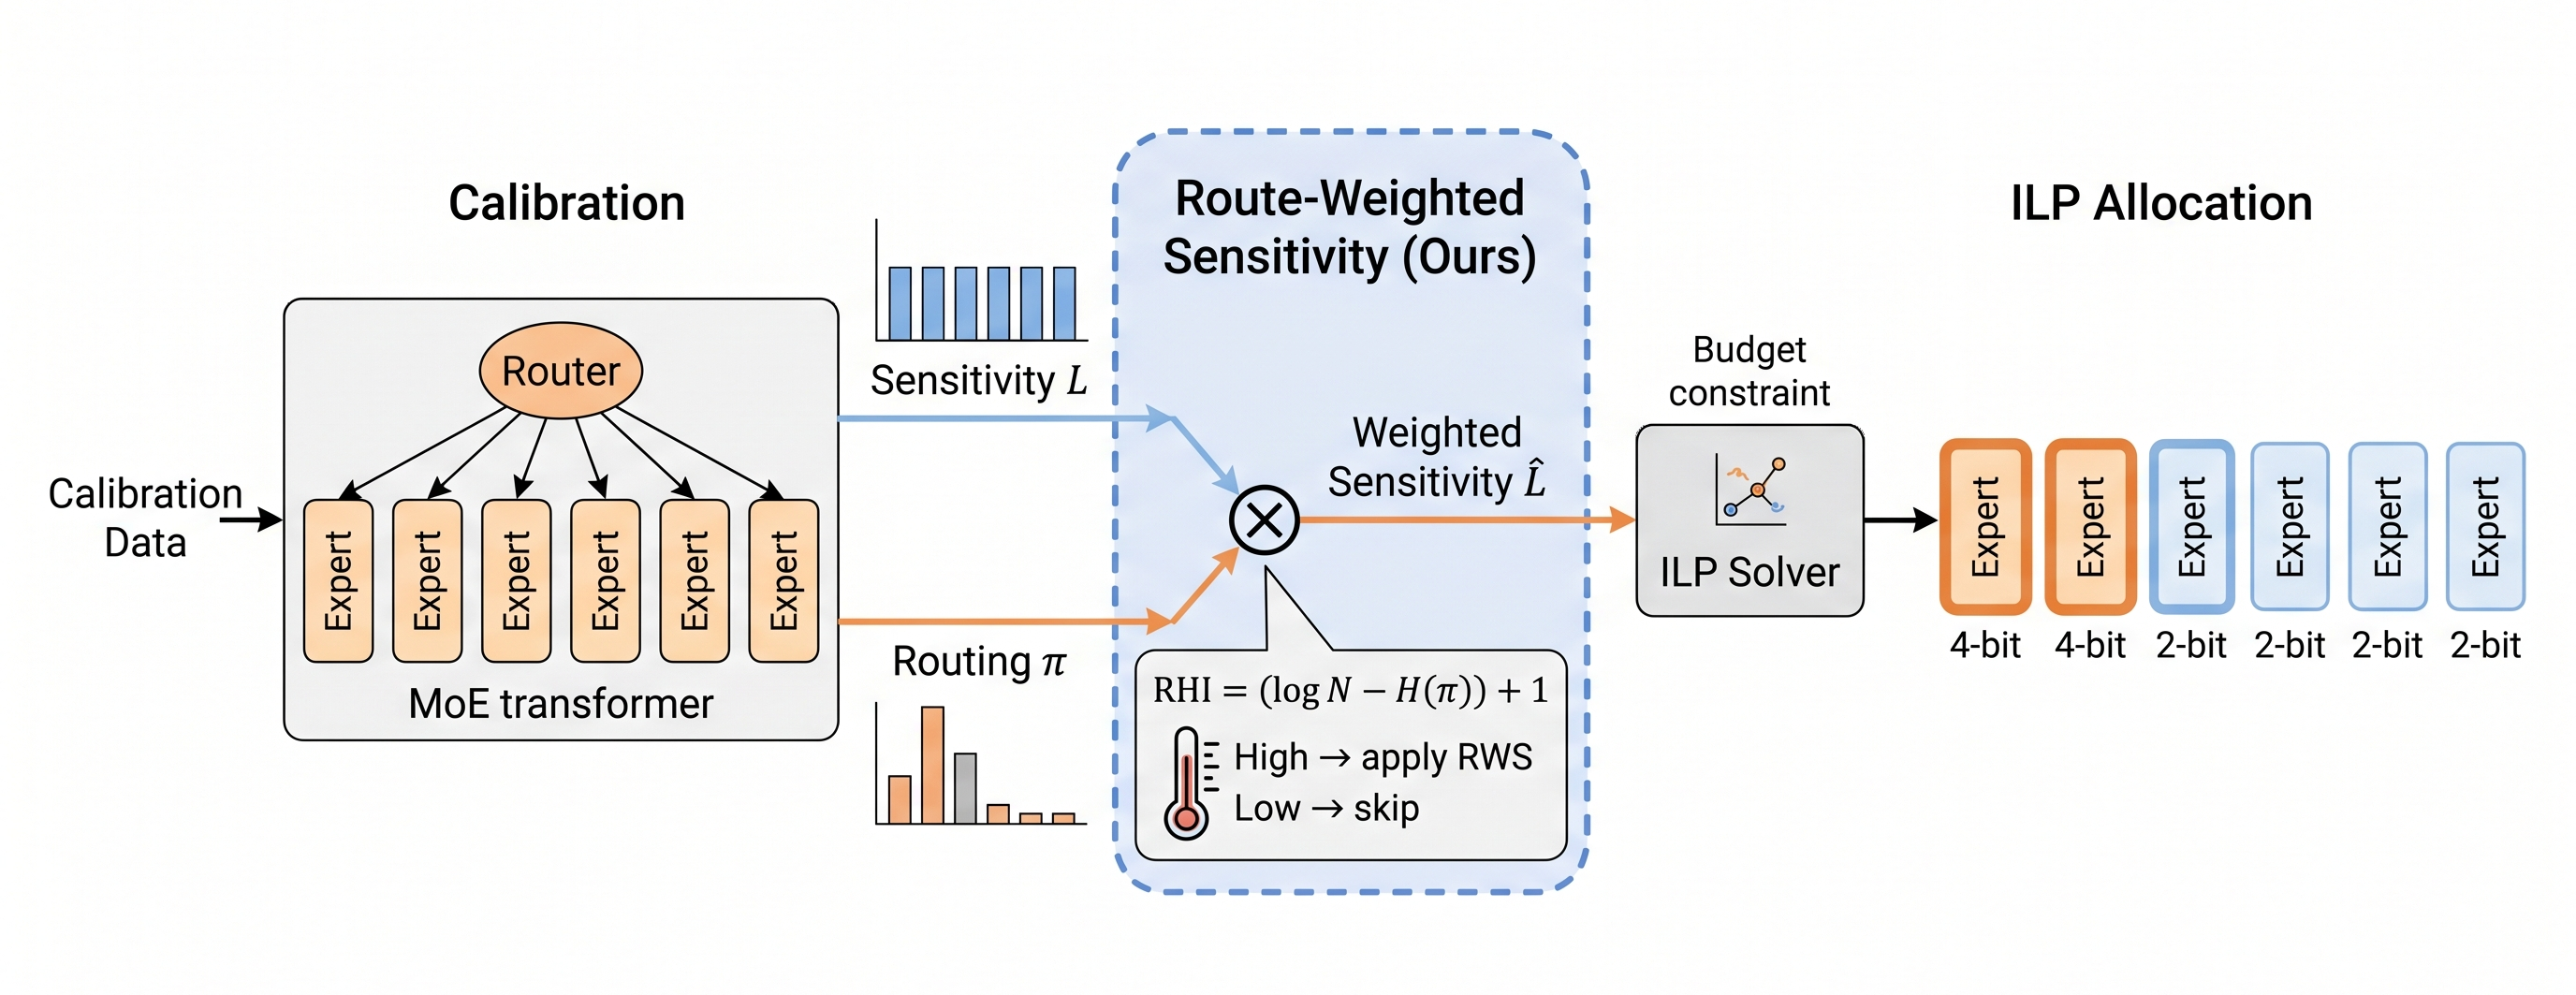
\includegraphics[width=0.95\textwidth]{figures/fig_framework.png}
\caption{Overview of \method. During the calibration forward pass, we collect both per-expert sensitivity scores $\Loss_{b,s}$ and routing probabilities $\piprob_{l,e}$. \method\ weights each expert's sensitivity by $\piprob_{l,e}$ before feeding it to the ILP allocator.}
\label{fig:framework}
\end{figure*}

\subsection{Route-Weighted Sensitivity}

Let $\piprob_{l,e} \in [0,1]$ denote the empirical routing probability of expert $e$ in layer $l$---the fraction of calibration tokens for which $e \in \mathcal{T}(x)$. Define the per-layer normalized routing weight:
\begin{equation}
\label{eq:weight}
  w_{l,e} \;=\; \frac{\piprob_{l,e}}{\max_{e'}\, \piprob_{l,e'}} \;\in\; [0,\, 1].
\end{equation}
We modify each block's sensitivity before the ILP by applying:
\begin{equation}
\label{eq:rws}
  \hat{\Loss}_{b,s} \;=\; \Loss_{b,s} \cdot \bigl(1 + w_{l(b),\,e(b)}\bigr).
\end{equation}
The $(1 + w)$ form ensures that high-frequency experts (with $w \approx 1$) receive approximately doubled sensitivity, while the lowest-frequency experts retain their original loss unchanged. The ILP then minimizes $\sum_{b,s} \hat{\Loss}_{b,s}\, x_{b,s}$ subject to the same constraints as Eq.~\ref{eq:ilp}. The substitution changes \emph{only} the objective; the constraints, strategy pool, solver, and calibration data are identical.

\paragraph{Loss computation.}
The calibration loss $\Loss_{b,s}$ is computed as follows. During the calibration forward pass, every expert processes \emph{all} calibration inputs regardless of routing. For each expert's linear block (gate, up, or down projection), we quantize the block weights to strategy $s$ and compute the $\ell_2$ reconstruction error $\|\hat{y} - y\|_2$ between the quantized and full-precision block outputs, averaged over the calibration sequence. This is an \emph{unconditional} per-block loss: it does not distinguish between tokens that are and are not routed to the expert. This distinction matters because the unconditional loss treats all blocks equally, while the expected inference loss weights each block by the probability that it is actually used. \method\ bridges this gap by scaling the unconditional loss by routing frequency.

\paragraph{Why $(1 + w)$ rather than raw $\piprob$.}
A theoretically cleaner objective would multiply by raw $\piprob_{l,e}$ to approximate the expected routed-token loss. We use the $(1 + w)$ form because it is conservative: it boosts high-frequency experts by at most $2\times$ and never reduces any expert's loss below its baseline. The $(1 + w)$ form recovers the baseline when routing is uniform ($w\!=\!1$ for all experts). While $(1 + w)$ and raw $\piprob$-weighting are both monotone in $\piprob$, they do not necessarily produce the \emph{same} ILP allocation in general, because the ILP's budget constraint creates tradeoffs across layers and blocks where the magnitude of the scaling---not just the ranking---affects which marginal block is promoted or demoted. In practice, we observe nearly identical allocations: on Qwen at 2.5\,bits, the two formulations differ in only 3 of 1,464 blocks.

\paragraph{Approximation caveat.}
The true conditional loss for expert $e$ is $\mathbb{E}_{x:\, e \in \mathcal{T}(x)}[\Loss_{e,s}(x)]$, which decomposes as $\Pr(e \in \mathcal{T}) \cdot \mathbb{E}_x[\Loss_{e,s}(x)]$ only when the quantization error is independent of whether $e$ is selected. When experts specialize \citep{zhou2022expertchoice}, this independence is imperfect. RWS is therefore a \emph{first-order approximation}. Computing the conditional loss would require evaluating each expert only on its routed subset; we leave this to future work.

\paragraph{Selection frequency vs.\ gate weight.}
We use $\piprob_{l,e} = \Pr(e \in \mathcal{T}(x))$ (top-$k$ selection frequency) rather than the expected gate weight $\alpha_{l,e} = \mathbb{E}_x[\mathbf{1}(e \in \mathcal{T}(x)) \cdot w_e(x)]$. The two are correlated but not identical; we choose $\piprob$ because it is simpler and produces nearly identical results (PPL 9.35 vs.\ 9.34 at 2.5\,b on Qwen). This ablation on Qwen shows that the specific choice of routing statistic matters less than the presence of routing information in the objective.

\paragraph{Shared experts.}
Models with shared experts (Qwen: 1 shared + 60 routed; DeepSeek: 2 shared + 64 routed) always activate their shared experts. Since shared experts have no routing decision, $\piprob$ is undefined for them. We apply route weighting \emph{only} to routed expert blocks, leaving shared expert sensitivities at their original values ($\hat{\Loss}_{b,s} = \Loss_{b,s}$). Mixtral has no shared experts, so all blocks are route-weighted.

\subsection{Route Heterogeneity Index}
\label{sec:rhi}

\method\ has leverage only when $\piprob$ is non-uniform. We quantify routing skew with the \emph{Route Heterogeneity Index}:
\begin{align}
\label{eq:rhi}
  \rhi_l &\;=\; \bigl(\log N - H(\piprob_l)\bigr) + 1, \\
  \rhi   &\;=\; \frac{1}{L}\sum_{l=1}^{L} \rhi_l,
\end{align}
where $H$ is Shannon entropy. The $+1$ shift makes $\rhi\!=\!1$ under uniform routing (a convenient baseline); without it, the metric would be the entropy deficit $\log N - H$, which carries the same information. Computing $\rhi$ takes milliseconds on a calibration trace.

\paragraph{Scope of the diagnostic.}
Three models provide insufficient evidence to validate $\rhi$ as a predictive diagnostic. Our three data points show that all models with $\rhi > 1$ benefit from RWS, and that the two models with higher $\rhi$ (Qwen and Mixtral, both 1.84) show PPL improvements of 2.8\% and 1.0\% at 2.5\,bits, while DeepSeek ($\rhi\!=\!1.56$) shows 1.3\%. Importantly, the two models with identical $\rhi$ show different gain magnitudes, indicating that $\rhi$ captures only one axis of variation---expert count, top-$k$, and model scale also mediate the effect. We present $\rhi$ as a preliminary diagnostic that practitioners can compute at negligible cost, not as a validated predictor.

\paragraph{Expected behavior.}
At slack budgets ($\ge\!3$\,bits), most blocks receive the high-bit strategy and reweighting has little leverage. At moderate budgets ($2.5$--$2.75$\,bits), the ILP must choose which blocks to promote, and $\piprob$-weighting shifts these promotions toward high-traffic experts. At extreme budgets ($\le\!2.3$\,bits), quantization dominates and few promotions are possible. \method\ should therefore help most in the aggressive regime---a prediction we verify in \S\ref{sec:results}.
